\documentclass[10pt,letterpaper]{article}
\usepackage[utf8]{inputenc}
\usepackage{amsmath}
\usepackage{amsfonts}
\usepackage{amssymb}
\usepackage{graphicx}
%\usepackage{algorithm}
%\usepackage{algpseudocode}

\newcommand{\R}{\mathbb{R}}
\renewcommand{\thesubsection}{\thesection.\alph{subsection}}

\author{Brock Ellefson, Seth Severa}
\title{CSCI432 GW5}

\begin{document}
\maketitle

\section{Find the Longest Nondecreasing Subsequence, what is the loop invariant? Note: be sure to fully justify.}
Our loop invariant L is: The longest nondecreasing substring A[0..i] is always greater than or equal to the longest nondecreasing substring of A[0..j]

\noindent If a loop invariant is true it must hold true to three conditions:
\begin{enumerate}
  \item $P \Rightarrow L$
  \item $L \wedge X \Rightarrow L$
  \item $L \wedge \sim X \Rightarrow Q$
\end{enumerate}
Where $P$ is our precondition, $X$ is our loop guard, and $Q$ is our postcondition.\\
\\
P implies L because upon entry of the loop, j is 0 and i is 1, which implies that our loop is true.\\
L and X implies L because while in the loop, our base case would be that the longest nondecreasing subsequence is the soley the first element, otherwise, we iterate through the loop. In each iteration, our j value will never be greater than our i value. Therefore A[0..j] will never be greater than A[0..i]\\
L and not X implies Q because once i equals A.size() we break our loop guard X (i $<$ A.size()) causing us to exit the loop with our longest nondecreasing subsequence 
\\
There our loop invariant L is true.

\subsection{Graph}
\begin{figure}[h]
	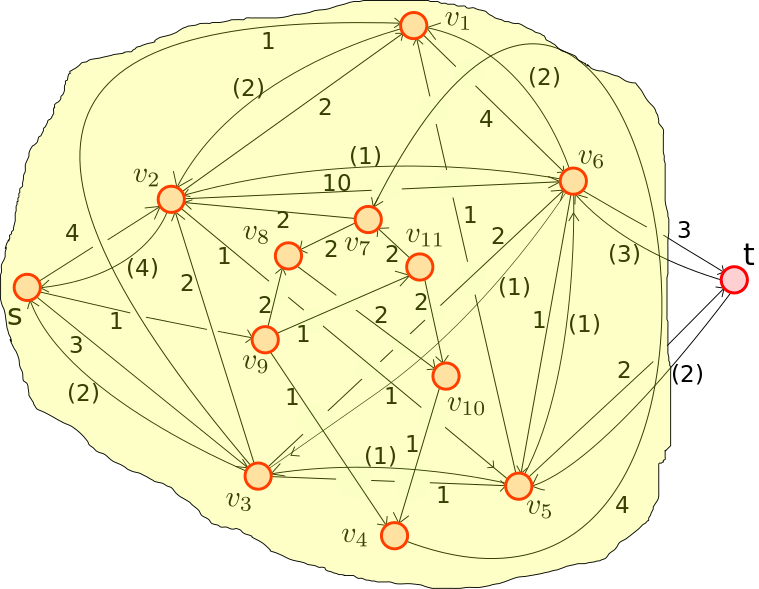
\includegraphics[scale = .5]{graph.png}
\section{Questions}
\subsection{What is the Euler characteristic of the graph?}
The Euler characteristic is $V - E \rightarrow 11 - 19 = -8$ 
\subsection{What is the graph genus?}
The graph genus of this graph is 13
\subsection{Is an Eulerian tour possible?}
A connected graph has an Eulerian cycle iff it has no graph vertices of odd degree.\\
This graph has multiple vertices with an odd of edges, therefore an Eulerian tour is not possible.

\subsection{Is a Hamiltonian path possible?}
A Hamiltonian path is possible. The path is as follows:\\
$v8 \rightarrow v10 \rightarrow v11 \rightarrow v9 \rightarrow v4 \rightarrow v7 \rightarrow v2 \rightarrow v3 \rightarrow v1 \rightarrow v6 \rightarrow v5$

\subsection{What is the size of the largest clique?}
The maximum clique is the clique of $v1$, $v2$, $v3$, $v5$, $v6$

\end{figure}
\end{document}
